\section{Theorie}
\label{sec:Theorie}
\subsection{Der Franck-Hertz-Versuch}
In \autoref{fig:aufbau} ist der Versuchsaufbau zum Franck-Hertz-Versuch schematisch dargestellt.

\begin{figure}[H]
    \centering
    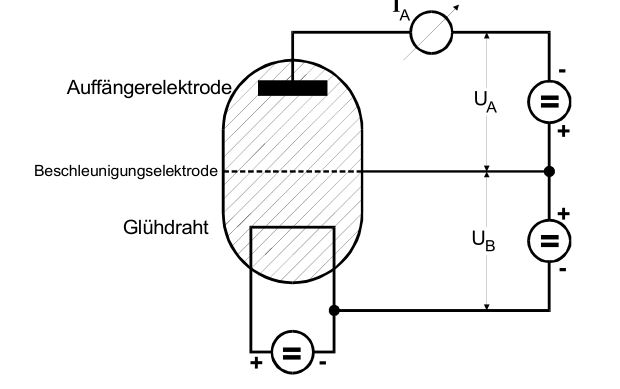
\includegraphics[width=\textwidth]{images/aufbau1.JPG}
    \caption{Schematischer Aufbau zum Franck-Hertz-Versuch. \cite{V601}}
    \label{fig:aufbau}
  \end{figure}
\noindent
Die Franck-Hertz-Apparatur besteht grundsätzlich aus einem evakuierten Gefäß mit einem Tropfen Quecksilber, welcher zum Verdampfen gebracht wird. In dem Glaskolben befindet sich ein Draht aus einem hochschmelzenden Metall, der stark erhitzt wird, sodass eine große Zahl von Elektronen aus dem Draht austreten. Dabei sollte der Draht mit dem Oxid eines Erdalkalimetalles bestrichen werden, da so aufgrund der niedrigeren Austrittsarbeit deutlich mehr freie Elektronen entstehen. Diese freien Elektronen werden dann mit einer Beschleunigungselektrode zu einer Auffängerelektrode beschleunigt. Nach dem Durchlaufen dieser Beschleunigungsstrecke, mit Beschleunigungsspannung $U_\text{B}$, haben die Elektronen also eine kinetische Energie von 

\begin{equation*}
    \frac{m_0}{2}v^2_\text{vor} = e_0 U_\text{B} \ .
\end{equation*}
\\
Um die Auffängerelektrode zu erreichen, benötigen die Elektronen dann mindestens die kinetische Energie
\begin{equation}
    \frac{m_0}{2}v^2_\text{z} \geq e_0 U_\text{A} \ .
    \label{eqn:energie}
\end{equation}
\\
Wenn es nun im Beschleunigungsraum zu Zusammenstößen zwischen den Hg-Atomen und den freien Elektronen kommt, treten zwei Fälle auf. Bei geringer Elektronenenergie $E$ treten elastische Stöße auf, bei denen aufgrund des großen Massenunterschiedes zwischen den Stoßpartnern nur eine geringe Energieabgabe von 
\begin{equation*}
    \symup{\Delta}E = \frac{4 m_0 M}{(m_0 + M)^2} E \approx \num{1.1e-5} E
\end{equation*}
zwischen Elektron und Hg-Atom auftritt. Wenn die Elektronenenergie aber mindestens der Energiedifferenz $E_1 - E_0$ zwischen dem 1. angeregten und
dem Grundzustand des Hg-Atoms entspricht, kann das Elektron das Hg-Atom anregen. Wenn das Hg-Atom dann wieder in seinen Grundzustand zurückgeht, wird es ein
Photon mit der Energie

\begin{equation*}
    E_\text{Photon} = h \nu = E_1 - E_0
\end{equation*}
emittieren. Idealerweise sieht der Zusammenhang vom Auffängerstrom $I_A$ in Abhängigkeit von der Beschleunigungsspannung $U_B$ wie in \autoref{verlauf} aus.
\begin{figure}[H]
    \centering
    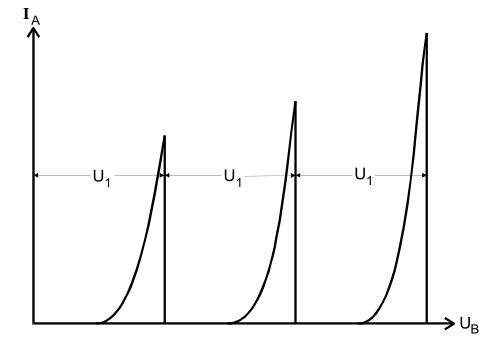
\includegraphics[width=\textwidth]{images/verlauf.JPG}
    \caption{Idealisierter Verlauf der Franck-Hertz-Kurve. \cite{V601}}
    \label{fig:verlauf}
  \end{figure}
\noindent
Die Abstände $U_1$ zwischen den Maxima des Auffängerstroms müssen dann dem 1.Anregunspotential
\begin{equation*}
      U_1 = \frac{1}{e_0} (E_1 - E_0)
  \end{equation*}
des Hg-Atoms entsprechen.

\subsection{Einflüsse auf die Form der Franck-Hertz-Kurve}
In diesem Abschnitt werden einige Einflüsse erläutert, die dazu führen, dass der idealisierte Verlauf der Franck-Hertz-Kurve aus \autoref{fig:verlauf} nicht erreicht wird.
\newline
\textbf{Das Kontaktpotential:}\newline
Aufgrund der Beschichtung des Glühdrahtes ist dessen Austrittsarbeit deutlich geringer als die Austrittsarbeit der Beschleunigungselektrode. In \autoref{fig:verh} ist das zwischen den Elektroden auftretende Potentialverhältnis dargestellt.
\begin{figure}[H]
    \centering
    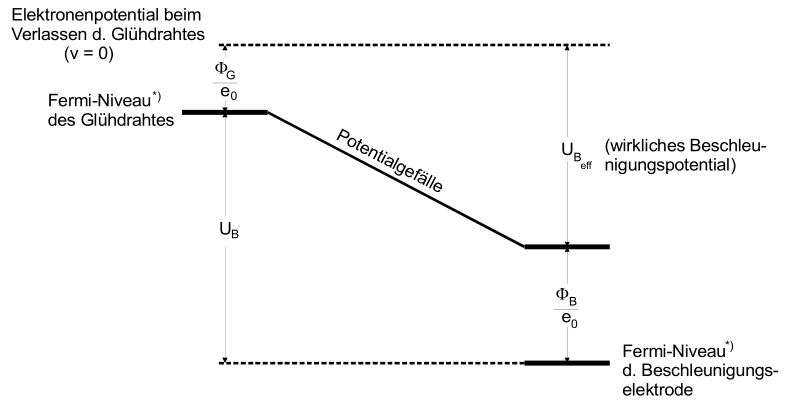
\includegraphics[width=\textwidth]{images/potential.JPG}
    \caption{Potentialverhältnis zwischen Glühkathode und Beschleunigungselektrode. \cite{V601}}
    \label{fig:verh}
  \end{figure}
\noindent
$\Phi_\text{G}$ und $\Phi_\text{B}$ sind dabei die Austrittsarbeiten von Draht und Beschleunigungselektrode. Aus diesen Potentialen lässt sich dann das Kontaktpotential
    \begin{equation*}
     K = \frac{1}{e_0} (\Phi_\text{B} - \Phi_\text{G}) 
    \end{equation*}
\noindent
bestimmen, welches zu einer Verschiebung der Franck-Hertz-Kurve um den Wert $K$ führt. \newline
\textbf{Das Energiespektrum der Elektronen:}\newline
Nach der Fermi-Dirac-Verteilung weisen die Elektronen im Glühdraht bereits vor dem Herauslösen verschiedene Energieniveaus auf, sodass sie nach der Beschleunigung ein kontinuierliches Energiespektrum besitzen. Aus diesem Effekt folgt, dass der Auffängerstrom nicht ganz auf Null abfallen wird,
sondern immer wieder einen Minimalwert größer 0 erreichen wird.\newline
\textbf{Der Dampfdruck:}\newline
Die Beobachtung der Franck-Hertz-Kurve ist nur möglich wenn ausreichend viele Zusammenstöße zwischen den Elektronen und den Hg-Atomen auftreten. Dies ist der Fall  wenn die mittlere freie Weglänge $\bar{w}$ der Atome klein gegen den Abstand a zwischen Kathode und Beschleunigungselektrode ist. $\bar{w}$ lässt sich über den Sättigungsdampfdruck $p_{\text{sät}}$ regeln und folgt dem Zusammenhang:
\begin{equation*}
    \bar w [cm] = \frac{0,0029}{p_{\text{sät}}} \;\text{[p in mbar]}
\end{equation*}
\noindent
Da der Sättigungsdampfdruck nur von der Temperatur T abhängt, kann aus dieser Gleichung berechnet werden, bei welchen Temperaturen der Franck-Hertz-Effekt beobachtbar ist. Dabei ist wichtig, dass $\bar{w}$ um das 1000- bis 4000-fache
kleiner als a sein muss, damit die Stoßwahrscheinlichkeit ausreichend hoch wird.